\section{Задача №6.1. Расчет виртуальной энтропии и теплоемкости}
\subsection{Постановка задачи}
\textit{Задача:} \textbf{рассчитать виртуальную энтропию $S_{\text{вирт}}$ и теплоемкости $C_{P}$ для вещества $NO_2$ при температуре $T=1700$ К и давлении $P=7$ атм.}

\subsection{Расчет виртуальной энтропии}
Виртуальную энтропию можно найти как сумму поступательной, вращательной и колебательной энтропий:
\begin{equation}
S_{\text{вирт}} = S_{\text{пост}} + S_{\text{вр}} + S_{\text{кол}},
\end{equation}
где $S_{\text{пост}}$, $S_{\text{вр}}$, $S_{\text{кол}}$ --- поступательная, вращательная и колебательная энтропия соответственно.

Для начала запишем некоторые параметры молекулы
\begin{table}[h!]
	\centering
	\caption{Данные о молекуле}
	\label{tab1}
	\setlength{\extrarowheight}{1mm}
\begin{tabular}{|c|c|}
	\hline 
	& $NO_2$ \\ 
	\hline 
	Длины связей, нм & $r_{N-O} = 0.1197$ \\ 
	\hline 
	Валентный угол & $\angle ONO = 134.3 \degree$ \\ 
	\hline 
	Частоты колебаний $\omega$, см$^{-1}$ & 1356, 757, 1664 \\ 
	\hline 
\end{tabular} 
\end{table}
\subsubsection{Расчет поступательной энтропии}
Поступательная энтропия для всех газообразных веществ рассчитывается по уравнению
\begin{equation}
S_{\text{пост}} = \left(\frac{3}{2}\,R\cdot \ln M+\frac{5}{2}\,R\cdot\ln T-R\cdot\ln P-9.7 \right) \cfrac{\text{Дж}}{\text{моль}\cdot\text{К}},
\end{equation}
где $M$ --- молекулярная масса в г/моль, $T$ --- температура системы в К, $P$ --- давление системы в атм.

$$
M = (14.0067+15.9994\cdot2) \text{ г/моль} = 46.0055 \text{ г/моль.}
$$

Таким образом
\begin{center}
	$S_{\text{пост}} = \left(\cfrac{3}{2} \cdot8.314\cdot \ln 46.0055+\cfrac{5}{2}\cdot 8.314\cdot\ln1700-8.314\cdot\ln 7-9.7 \right) \cfrac{\text{Дж}}{\text{моль}\cdot\text{К}} = 176.48\  \cfrac{\text{Дж}}{\text{моль}\cdot\text{К}}.$
\end{center}
Итак,
\begin{equation}
\boxed{S_{\text{пост}} = 176.48\  \cfrac{\text{Дж}}{\text{моль}\cdot\text{К}}}.
\end{equation}
\subsubsection{Расчет вращательной энтропии}
Вращательная энтропия для всех нелинейных молекул определяется по уравнению
\begin{equation}
S_{\text{вр}} = \left(\cfrac{1}{2}\,R\cdot\ln I_1I_2I_3+\cfrac{3}{2}\,R\cdot\ln T - R\cdot\ln\sigma+1320.8\right)\cfrac{\text{Дж}}{\text{моль}\cdot\text{К}},
\end{equation}
где $I_1$, $I_2$, $I_3$ --- главные значения тензора момента инерции многоатомной нелинейной молекулы, выражены в кг$\cdot$м$^2$, $\sigma$ --- число симметрии молекулы.

Для расчета произведения главных моментов тензора момента инерции воспользуемся методом Хиршфельдера
\begin{equation}
I_1I_2I_3 = \begin{vmatrix}
A & -D & -E\\
-D & B & -F\\
-E & -F & C\\
\end{vmatrix}
= ABC -AF^2-BE^2-CD^2-2DFE.
\end{equation}
В этой формуле
\begin{center}
	$
	A = \sum\limits_i m_i(y_i^2+z_i^2) - \cfrac{1}{\overline m}\left(\sum\limits_im_iy_i\right)^2- \cfrac{1}{\overline m}\left(\sum\limits_im_iz_i\right)^2$,\\
	$B = \sum\limits_i m_i(x_i^2+z_i^2) - \cfrac{1}{\overline m}\left(\sum\limits_im_ix_i\right)^2- \cfrac{1}{\overline m}\left(\sum\limits_im_iz_i\right)^2$,\\
	$C = \sum\limits_i m_i(x_i^2+y_i^2) - \cfrac{1}{\overline m}\left(\sum\limits_im_ix_i\right)^2- \cfrac{1}{\overline m}\left(\sum\limits_im_iy_i\right)^2$,\\
	$
	D = \sum\limits_im_ix_iy_i - \cfrac{1}{\overline m} \left(\sum\limits_im_ix_i\right)\left(\sum\limits_im_iy_i\right)$,\\	
	$
	E = \sum\limits_im_ix_iz_i - \cfrac{1}{\overline m} \left(\sum\limits_im_ix_i\right)\left(\sum\limits_im_iz_i\right)$,\\
	$
	F = \sum\limits_im_iy_iz_i - \cfrac{1}{\overline m} \left(\sum\limits_im_iy_i\right)\left(\sum\limits_im_iz_i\right)$,\\
	$\overline m = \sum\limits_i m_i$,
\end{center}
где $m_i$ --- масса, $x_i$, $y_i$, $z_i$ --- декартовы координаты i-го атома.

Расположим молекулу $NO_2$ так, как показано на рисунке \ref{fig:geogebra-export}. 
\begin{figure}
	\centering
	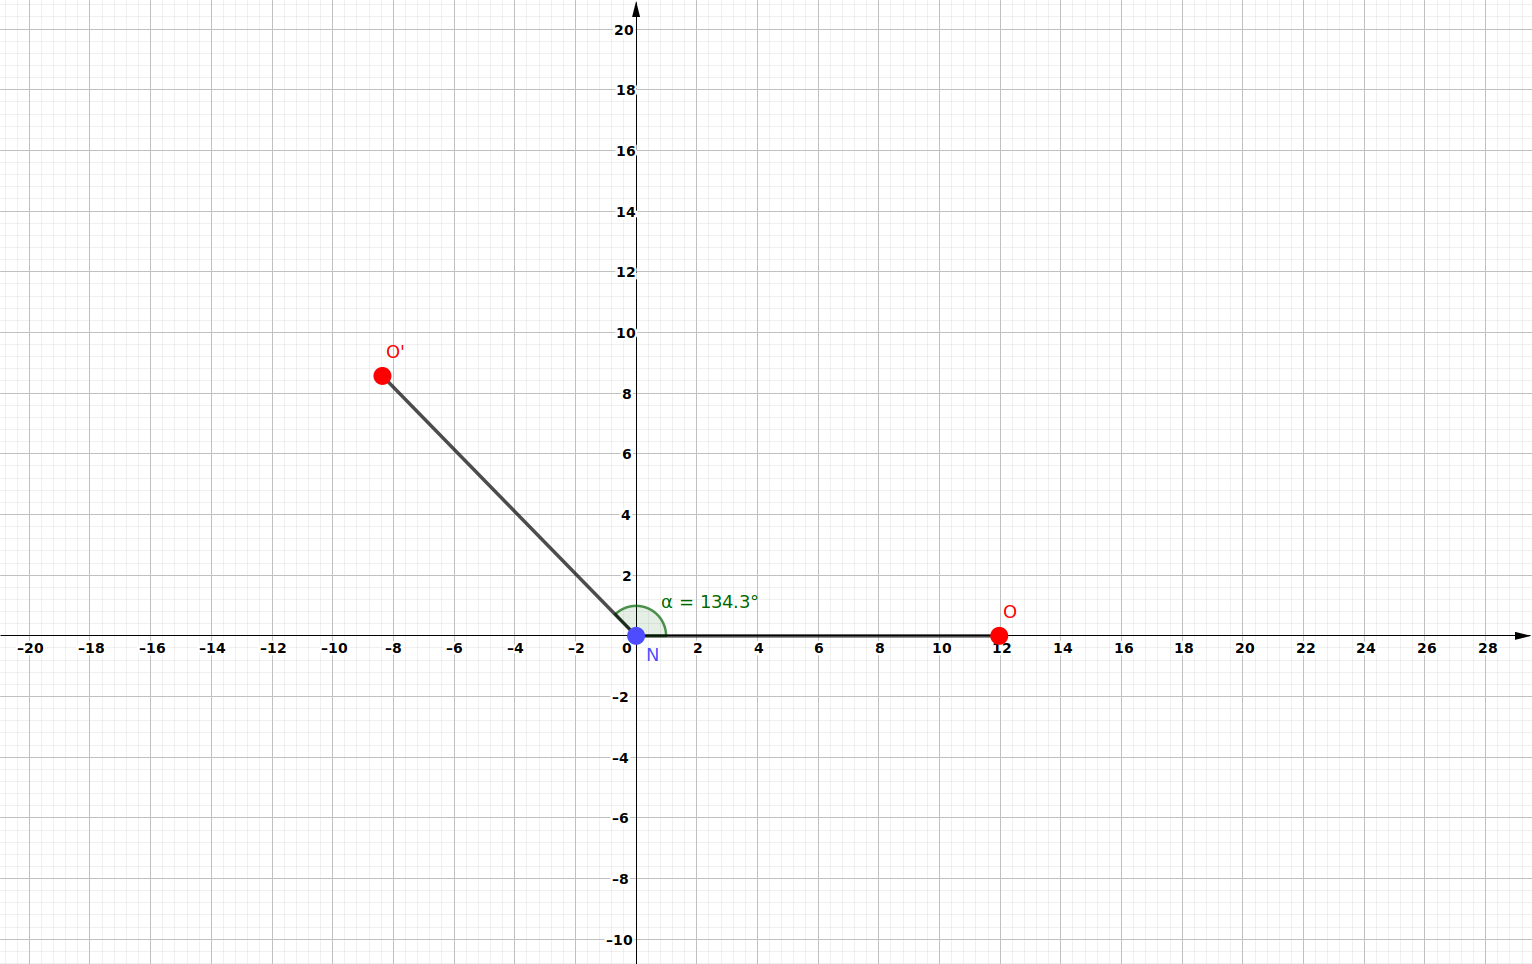
\includegraphics[width=0.7\linewidth]{geogebra-export}
	\caption{}
	\label{fig:geogebra-export}
\end{figure}

%TODO надо сделать рисунок
Тогда при выбранном начале координат и направлениях осей координаты осей будут следующими
\begin{table}[h!]
	\centering
	\caption{Координаты атомов}
	\label{tab3}
	\setlength{\extrarowheight}{1mm}
	\begin{tabular}{|c|c|c|c|}
		\hline 
		Атом & $x$, нм & $y$, нм & Масса атома, кг \\ 
		\hline 
		$N$ & 0 & 0 & $2.32\cdot10^{-26}$ \\ 
		\hline 
		$O$ & 0.1197 & 0 & $2.66\cdot10^{-26}$ \\ 
		\hline 
		$O$ & -0.0836 & 0.0857 & $2.66\cdot10^{-26}$ \\ 
		\hline 
	\end{tabular} 
\end{table}

Тогда в нашем случае
\begin{equation}
I_1I_2I_3 = \begin{vmatrix}
A & -D & 0\\
-D & B & 0\\
0 & 0 & C\\
\end{vmatrix}
= C(AB-D^2).
\end{equation}
Найдем выражения для компонент определителя
\begin{center}
	$\overline m = \cfrac{46.0055\cdot10^{-3}}{6.02\cdot10^{23}} = 7.64\cdot10^{-26}$ кг;\\
	$	A = \sum\limits_i m_iy_i^2 - \cfrac{1}{\overline m}\left(\sum\limits_im_iy_i\right)^2 = 2.66\cdot10^{-26}\,(8.567\cdot10^{-11})^2-\cfrac{1}{7.64\cdot10^{-26}}\left(2.66\cdot10^{-26}\,8.567\cdot10^{-11}\right)^2 = 1.95\cdot10^{-46}$ кг$\cdot$м$^2$;\\
	$B = \sum\limits_i m_ix_i^2 - \cfrac{1}{\overline m}\left(\sum\limits_im_ix_i\right)^2 = 2.66\cdot10^{-26}\,((11.97\cdot10^{-11})^2+(-8.36\cdot10^{-11})^2)-\cfrac{1}{7.64\cdot10^{-26}}\left(2.66\cdot10^{-26}\,\left(11.97\cdot10^{-11}-8.36\cdot10^{-11}\right)\right)^2 = 5.67\cdot10^{-46}$ кг$\cdot$м$^2$;\\
	$C = \sum\limits_i m_i(x_i^2+y_i^2) - \cfrac{1}{\overline m}\left(\sum\limits_im_ix_i\right)^2- \cfrac{1}{\overline m}\left(\sum\limits_im_iy_i\right)^2 =
	2.66\cdot10^{-26}\,((11.97\cdot10^{-11})^2+(-8.36\cdot10^{-11})^2+(8.567\cdot10^{-11})^2)-\cfrac{1}{7.64\cdot10^{-26}}\left(2.66\cdot10^{-26}\,\left(11.97\cdot10^{-11}-8.36\cdot10^{-11}\right)\right)^2 -\cfrac{1}{7.64\cdot10^{-26}}\left(2.66\cdot10^{-26}\,8.567\cdot10^{-11}\right)^2= 7.61\cdot10^{-46}$ кг$\cdot$м$^2$;\\
	$D = \sum\limits_im_ix_iy_i - \cfrac{1}{\overline m} \left(\sum\limits_im_ix_i\right)\left(\sum\limits_im_iy_i\right) = 
	2.66\cdot10^{-26}\,8.567\cdot(-8.36)\cdot10^{-22}-\cfrac{1}{7.64\cdot10^{-26}}\left(2.66\cdot10^{-26}\, (11.97\cdot10^{-11}-8.36\cdot10^{-11})\right)\cdot\left(2.66\cdot10^{-26}\,8.567\cdot10^{-11}\right) = -1.903\cdot10^{-46}$ кг$\cdot$м$^2$.
\end{center}
В итоге
$$
I_1I_2I_3 = 7.61(1.95\cdot5.67-1.903^2)\cdot10^{-138} = 5.67\cdot10^{-137}.
$$

Данная молекула обладает одной осью симметрии второго порядка, откуда
$$
\sigma = 2.
$$
Таким образом
\begin{center}
	$S_{\text{вр}} = \left(\cfrac{1}{2}\,8.314\cdot\ln (5.67\cdot10^{-137})+\cfrac{3}{2}\,8.314\cdot\ln 1700 - 8.314\cdot\ln2+1320.8\right)\cfrac{\text{Дж}}{\text{моль}\cdot\text{К}}= 103.67\ \cfrac{\text{Дж}}{\text{моль}\cdot\text{К}}$
\end{center}

Итак,
\begin{equation}
\boxed{S_{\text{вр}} = 103.67\  \cfrac{\text{Дж}}{\text{моль}\cdot\text{К}}}.
\end{equation}
\subsubsection{Расчет колебательной энтропии}
При расчете колебательной составляющей энтропии выдвинуто приближение, заключающееся в том, что молекула представлена в виде жёсткого гармонического осциллятора.

Для того, чтобы посчитать вклад $S_{i, \text{кол}}$ от каждой частоты, воспользуемся формулой
\begin{equation}
S_{i, \text{кол}} = R\,\cfrac{\frac{h\nu_i}{kT}}{e^{\frac{h\nu_i}{kT}}-1}-R\ln(1-e^{-\frac{h\nu_i}{kT}}),
\end{equation} 
или, записав ее в более удобном виде,
\begin{equation}
S_{i, \text{кол}} = R\,\cfrac{\frac{\theta_i}{T}}{e^{\frac{\theta_i}{T}}-1}-R\ln(1-e^{-\frac{\theta_i}{T}}),
\end{equation}
где $\theta_i$ --- характеристическая температура $i$-ой частоты колебаний. 

Для перевода волнового числа $\omega$ в $\theta$ надо величину $\omega$ умножить на коэффициент $\frac{ch}{k} = 1.438$, где $c$ --- скорость света, $h$ --- постоянная Планка, $k$ --- постоянная Больцмана.

Составим для удобства расчетов таблицу.
\begin{table}[h!]
	\centering
	\caption{Колебательная энтропия}
	\label{tab2}
	\setlength{\extrarowheight}{1mm}
	\begin{tabular}{|c|c|c|c|}
		\hline
		$\omega$, см$^{-1}$ & $\theta$, К & $\frac{\theta}{T}$ & $S_{i,\text{кол}}$, $\frac{\text{Дж}}{\text{моль}\cdot\text{К}}$ \\
		\hline 
		1356 & 1950 & 1.15 & 7.61 \\ 
		\hline 
		757 & 1089 & 0.64 & 12.16 \\ 
		\hline 
		1664 & 2393 & 1.41 & 6.13 \\ 
		\hline 
		\multicolumn{3}{|c|}{} & $\sum\limits_i S_{i,\text{кол}} = 25.90$ \\ 
		\hline 
		\end{tabular} 
\end{table}

Итак,
\begin{equation}
\boxed{S_{\text{кол}} = 25.90\  \cfrac{\text{Дж}}{\text{моль}\cdot\text{К}}}.
\end{equation}
\subsubsection{Окончательное значение виртуальной энтропии}
Таким образом, виртуальная энтропия $NO_2$ равна
\begin{center}
$S_{\text{вирт}} = S_{\text{пост}} + S_{\text{вр}} + S_{\text{кол}} = 176.48+103.67+25.90 = 306.05\ \cfrac{\text{Дж}}{\text{моль}\cdot\text{К}}$
\end{center}
Итоговый результат
\begin{equation}
\boxed{S_{\text{вирт}} = 306.05\  \cfrac{\text{Дж}}{\text{моль}\cdot\text{К}}}.
\end{equation}

\subsection{Расчет теплоемкости $C_P$}
Теплоемкость $C_P$ можно найти как сумму поступательной, вращательной и колебательной теплоемкостей
\begin{equation}
C_P = C_{\text{пост}} + C_{\text{вр}} + C_{\text{кол}},
\end{equation}
где $C_{\text{пост}}$, $C_{\text{вр}}$, $C_{\text{кол}}$ --- поступательная, вращательная и колебательная теплоемкость соответственно.

Найти $C_{\text{пост}}$ и $C_{\text{вр}}$ не составляет труда (молекула $NO_2$ не является линейной)
\begin{equation}
C_{\text{пост}} = \cfrac{5}{2}\,R \qquad C_{\text{вр}} = \cfrac{3}{2}R.
\end{equation}

Для расчета колебательной теплоемкости воспользуемся формулой
\begin{equation}
C_{i,\text{кол}} =R\, \cfrac{\left(\frac{\theta_i}{T}\right)^2e^{\frac{\theta_i}{T}}}{\left(e^{\frac{\theta_i}{T}}-1\right)^2}.
\end{equation}

Составим для удобства расчетов таблицу.

\begin{table}[h!]
	\centering
	\caption{Колебательная теплоемкость}
	\label{tab2}
	\setlength{\extrarowheight}{1mm}
	\begin{tabular}{|c|c|c|c|}
		\hline
		$\omega$, см$^{-1}$ & $\theta$, К & $\frac{\theta}{T}$ & $C_{i,\text{кол}}$, $\frac{\text{Дж}}{\text{моль}\cdot\text{К}}$ \\
		\hline 
		1356 & 1950 & 1.15 & 7.46 \\ 
		\hline 
		757 & 1089 & 0.64 & 8.03 \\ 
		\hline 
		1664 & 2393 & 1.41 & 7.07 \\ 
		\hline 
		\multicolumn{3}{|c|}{} & $\sum\limits_i C_{i,\text{кол}} = 22.56$ \\ 
		\hline 
	\end{tabular} 
\end{table}

Таким образом
$$
C_P = C_{\text{пост}} + C_{\text{вр}} + C_{\text{кол}} = \cfrac{5}{2}\,8.314 + \cfrac{3}{2}\,8.314+22.56 = 55.82\ \frac{\text{Дж}}{\text{моль}\cdot\text{К}}
$$

Итоговый результат
\begin{equation}
\boxed{C_P = 55.82\  \cfrac{\text{Дж}}{\text{моль}\cdot\text{К}}}.
\end{equation}

\subsection{Сопоставление результата с уравнением энтропии}
Сопоставим результаты расчета с уравнением
\begin{equation}
S = S_{298}^0 + \int\limits_{298}^{1700}\cfrac{C_P(T) dT}{T}-R\ln P = 306.94,
\end{equation}
где $C_P(T) = C_{\text{пост}} + C_{\text{вр}} + C_{\text{кол}}(T)$, $S_{298}^0 = 240.45\ \frac{\text{Дж}}{\text{моль}\cdot\text{К}}. $ 

Подставив все значения, получим
\begin{multline}
S = 240.45  + \\ + \int\limits_{298}^{1700}\left(\frac{(1950/T)^2\cdot e^{\frac{1950}{T}}}{(e^{\frac{1950}{T}}-1)^2}+\frac{(1089/T)^2\cdot e^{\frac{1089}{T}}}{(e^{\frac{1089}{T}}-1)^2}+\frac{(2393/T)^2\cdot e^{\frac{2393}{T}}}{(e^{\frac{2393}{T}}-1)^2}+4\right)\cdot\cfrac{8.314}{T}\,dT  - \\  -8.314\cdot\ln7 = 306.94 \ \cfrac{\text{Дж}}{\text{моль}\cdot\text{К}}
\end{multline}

Итак,
\begin{equation}
\boxed{S = 306.94 \ \cfrac{\text{Дж}}{\text{моль}\cdot\text{К}}}.
\end{equation}

Можно видеть, что величины $S$ и $S_{\text{вирт}}$ находятся в достаточном согласии друг с другом.









